% Options for packages loaded elsewhere
\PassOptionsToPackage{unicode}{hyperref}
\PassOptionsToPackage{hyphens}{url}
%
\documentclass[
]{book}
\usepackage{amsmath,amssymb}
\usepackage{lmodern}
\usepackage{iftex}
\ifPDFTeX
  \usepackage[T1]{fontenc}
  \usepackage[utf8]{inputenc}
  \usepackage{textcomp} % provide euro and other symbols
\else % if luatex or xetex
  \usepackage{unicode-math}
  \defaultfontfeatures{Scale=MatchLowercase}
  \defaultfontfeatures[\rmfamily]{Ligatures=TeX,Scale=1}
\fi
% Use upquote if available, for straight quotes in verbatim environments
\IfFileExists{upquote.sty}{\usepackage{upquote}}{}
\IfFileExists{microtype.sty}{% use microtype if available
  \usepackage[]{microtype}
  \UseMicrotypeSet[protrusion]{basicmath} % disable protrusion for tt fonts
}{}
\makeatletter
\@ifundefined{KOMAClassName}{% if non-KOMA class
  \IfFileExists{parskip.sty}{%
    \usepackage{parskip}
  }{% else
    \setlength{\parindent}{0pt}
    \setlength{\parskip}{6pt plus 2pt minus 1pt}}
}{% if KOMA class
  \KOMAoptions{parskip=half}}
\makeatother
\usepackage{xcolor}
\IfFileExists{xurl.sty}{\usepackage{xurl}}{} % add URL line breaks if available
\IfFileExists{bookmark.sty}{\usepackage{bookmark}}{\usepackage{hyperref}}
\hypersetup{
  pdftitle={History},
  pdfauthor={Dyrehaugen Web Notebook},
  hidelinks,
  pdfcreator={LaTeX via pandoc}}
\urlstyle{same} % disable monospaced font for URLs
\usepackage{longtable,booktabs,array}
\usepackage{calc} % for calculating minipage widths
% Correct order of tables after \paragraph or \subparagraph
\usepackage{etoolbox}
\makeatletter
\patchcmd\longtable{\par}{\if@noskipsec\mbox{}\fi\par}{}{}
\makeatother
% Allow footnotes in longtable head/foot
\IfFileExists{footnotehyper.sty}{\usepackage{footnotehyper}}{\usepackage{footnote}}
\makesavenoteenv{longtable}
\usepackage{graphicx}
\makeatletter
\def\maxwidth{\ifdim\Gin@nat@width>\linewidth\linewidth\else\Gin@nat@width\fi}
\def\maxheight{\ifdim\Gin@nat@height>\textheight\textheight\else\Gin@nat@height\fi}
\makeatother
% Scale images if necessary, so that they will not overflow the page
% margins by default, and it is still possible to overwrite the defaults
% using explicit options in \includegraphics[width, height, ...]{}
\setkeys{Gin}{width=\maxwidth,height=\maxheight,keepaspectratio}
% Set default figure placement to htbp
\makeatletter
\def\fps@figure{htbp}
\makeatother
\setlength{\emergencystretch}{3em} % prevent overfull lines
\providecommand{\tightlist}{%
  \setlength{\itemsep}{0pt}\setlength{\parskip}{0pt}}
\setcounter{secnumdepth}{5}
\usepackage{booktabs}
\usepackage{amsthm}
\makeatletter
\def\thm@space@setup{%
  \thm@preskip=8pt plus 2pt minus 4pt
  \thm@postskip=\thm@preskip
}
\makeatother

\renewcommand\chaptername{}
\ifLuaTeX
  \usepackage{selnolig}  % disable illegal ligatures
\fi
\usepackage[]{natbib}
\bibliographystyle{apalike}

\title{History}
\author{Dyrehaugen Web Notebook}
\date{2023-09-08}

\begin{document}
\maketitle

{
\setcounter{tocdepth}{1}
\tableofcontents
}
\hypertarget{history}{%
\chapter{History}\label{history}}

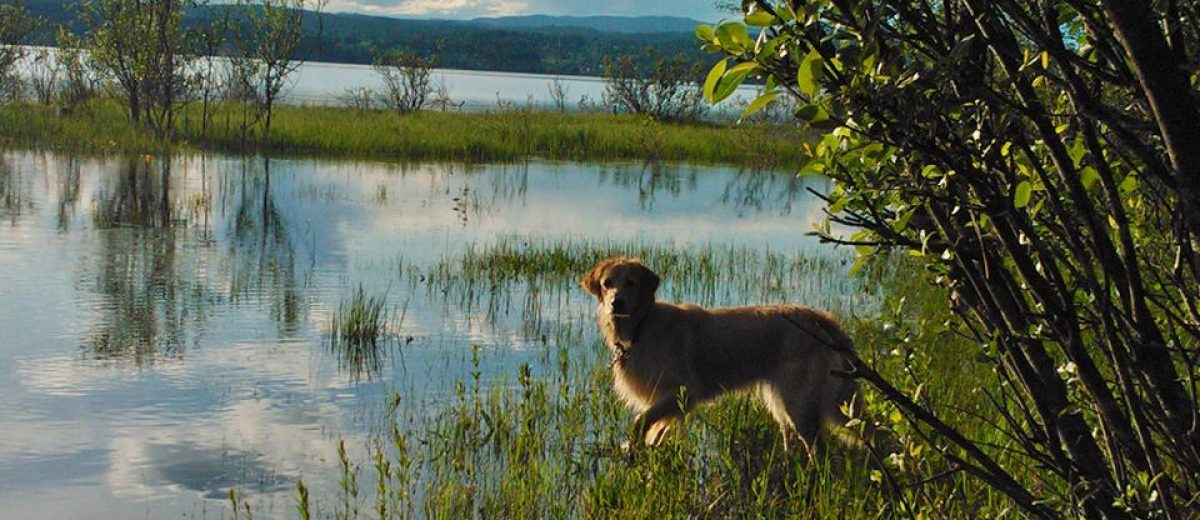
\includegraphics{fig/zelda.jpg}

\hypertarget{russia}{%
\chapter{Russia}\label{russia}}

\emph{Feygin}

One of the \href{https://www.jstor.org/stable/41051747}{big debates} in the historiography of the USSR is the so-called ``neo-traditionalist'' versus ``alternative modernity'' schools. Neo-traditionalists argue that the USSR should be understood in the context of a broader continuity of Russian historical trends. They tend to be social historians who look at the persistence of practices like the economy of favors and see a state that, whatever its intentions, operates through the habits of Edward Keenan's concept of \href{https://www.jstor.org/stable/130423}{``Muscovite Political Folkways.''} On the other hand, scholars who subscribe to the multiple modernities framework tend to study the USSR as a variant of the modernist state, with roots in the Western enlightenment tradition and the broader global political conjuncture. These tend to be historians influenced by the cultural turn and thus often examine how Soviet social relations are created by the subject's engagement with what Steve Kotkin called the ``grand strategy of the state.'' In turn, the USSR is not something outside of the modern experience but a specific variety of modernity: one amongst many. There are, of course, many debates within these paradigms and nuances, but this is the rough idea.

Interestingly, this whole debate is mostly about the Stalin era and, even more specifically, pre-war Stalinism. The post-war, post-Soviet, and late-Soviet periods don't play into things that much. This is because of how the field evolved over time and because the bedrock question for these histories is the legacy of 1917: how that revolution turned into that regime? Was it an inevitable result of Leninism, or was it something particular to Russia's social structure?

What things like understanding Wagner as a PE firm force us to do is not only go beyond the usual timeframe of this debate but also make some assumptions very explicit. First, it has to contend with \href{https://www.ghi-dc.org/fileadmin/publications/Bulletin_Supplement/Supplement_14/Sup14_105.pdf}{modernity as a moving target}, one that the USSR's existence shaped. Is the Cold War part of modernity or post-modernity? Is the American hegemonic system the same as the European Imperial one that the USSR was born under? Maybe that was easier to put aside in the 1990s when these debates began, but it is not so easy now. Second, we should have a very thick and explicit distinction between ``micro'' and ``macro.'' Historians hate theory, but the micro-macro distinction, even if it is reductionist, does help other social scientists have a language about causality. Do we have to root our model of the world on some micro actor's rationality, or do macro conditions themselves form the concept of rationality is as much a debate in economics (well, not in the mainstream of the field but increasingly more so) as it is in the \href{https://www.jstor.org/stable/41052991}{Soviet subjectivity debate} within the multiple modernities approach (whether there is some subject that rationally reacts to ideological projects or whether we should not see these reactions as a cost-benefit analysis and examine belief as an articulation of genuine beliefs).

Why I find this thought about the Concord group and violent PE so intriguing is that it offers us a way to look at the Russian state through the lens of political economy: that is to ask how it has adapted very liberal institutions like a private equity firm to very illiberal means. This does not mean that Russia or the USSR is some perversion of or final boss of modernity. Nor that it is traditionalist and guided by folkways more or less than any other society. Rather, it is a set of elites with tools that they adapt to do something at a certain cost and with some form of leverage that is structured via lots of complex path dependencies and constraints. Concord Group's adaptation of the PE model, by some accounts, the ultimate representative of globalist neoliberalism to achieve the Russian state's very un-globalized Great Power political ends provides a lot of food for thought.

\href{https://building-a-ruin.ghost.io/wagner-political-economy-historiography}{Feygin (2023) Wagner Group, Private Equity, Historiography}

\href{pdf/Krylova_2017_History_of_The_Soviet.pdf}{Kylova (2017) History of The `Soviet' (pdf)}

\hypertarget{usa}{%
\chapter{USA}\label{usa}}

\emph{Smith}

In the late 80s and 90s, it felt like we were on the cusp of a great shift, where the back-slapping jocks who had dominated American society in earlier times were on the verge of losing power and status to the bespectacled freaks and geeks. The Revenge of the Nerds was coming.

It wasn't just fantasy, either. Over the next thirty years, the nerds really did win the economic competition. The U.S. shifted from manufacturing to knowledge industries like IT, finance, bio, and so on, effectively going from the world's workshop to the world's research park. This meant that simply being able to cut deals and manage large workforces were no longer the only important skills you needed to succeed at the highest levels of business. Bespectacled programmers and math nerds became our richest men. From the early 80s to the 2000s, the college earnings premium rose relentlessly, and a degree went from optional to almost mandatory for financial success.
The age of human capital was in full swing, and the general consensus was that ``Average Is Over''.

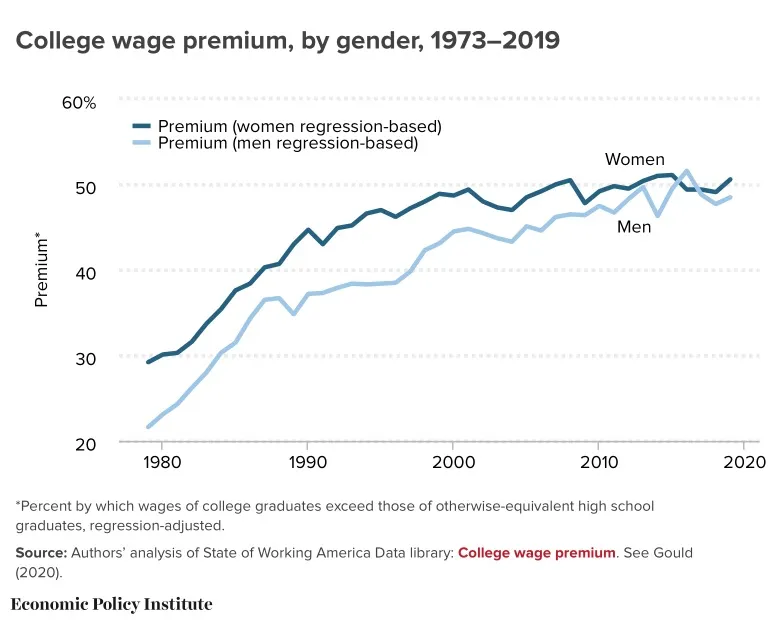
\includegraphics{fig/US_College_Wage_Premium_1980-2020.png}

That trend lasted so long that most Americans can no longer remember anything else. We've become used to the idea that technology brings inequality, by delivering outsized benefits to the 20\% of society who are smart and educated enough to take full advantage of it. It's gotten to the point where we tacitly assume that this is just what technology does, period, so that when a new technology like generative AI comes along, people leap to predict that economic inequality will widen as a result of a new digital divide.

And it's possible that will happen. I can't rule it out. But I also have a more optimistic take here --- I think it's possible that the wave of new technologies now arriving in our economy will decrease much of the skills gap that opened up in the decades since 1980.

\textbf{AI coming}

A whole lot of research is being done on the productivity effects of generative AI tools, and they all seem to conclude the same thing: Generative AI gives a much bigger boost to low performers than to high performers.

No study so far showing that more talented people are able to use generative AI more effectively than less talented people. All of the evidence points to generative AI as an equalizer.

It's not hard to think of why this might be the case. Whereas previous forms of information technology complemented human cognition, generative AI tends to substitute for human cognition.

Traditional IT acted like a shovel --- something that complemented people's natural abilities --- while generative AI acts more like a steam shovel. A steam shovel handles the muscle-power for you; GPT-4 handles the detail-oriented thinking for you. Technologies that substitute for natural ability tend to make natural ability less scarce, and therefore less valuable.

This doesn't mean generative AI will decrease inequality overall. The computation-intensive nature of these tools means that physical capital --- access to large amounts of cheap GPUs or other key hardware --- might make a comeback as a source of wealth. But by boosting the performance of the least skilled on cognitive tasks, generative AI looks like it could level the human-capital playing field.

\href{https://www.noahpinion.blog/p/is-it-time-for-the-revenge-of-the}{Smith (2023) Is it time for the Revenge of the Normies}

\hypertarget{part-appendices}{%
\part{Appendices}\label{part-appendices}}

\hypertarget{appendix-appendices}{%
\appendix}


\hypertarget{about}{%
\chapter{About}\label{about}}


\includegraphics{fig/me.jpg}

\emph{Dyre Haugen} and \emph{Dyrehaugen} is Webian for \emph{Jon Martin} -
self-owned Globian, Webian, Norwegian and Canarian with
a background from industrial research policy, urban planning and
economic development consulting on global, regional and urban scales.
I am deeply concerned about the (insane) way
humanity (i.e.~capitalism) interfere with nature.
In an effort to gain insights in how and why this happens
stuff is collected from around the web and put together
in a linked set of web-sites.
The sites are operated as personal notebooks.
However, these days things can be easily published to the
benefit of others concerned with the same issues.
But be aware - this is not polished for presentation or
peer-reviewed for exactness.
I offer you just to have a look at my `work-desk' as it appears in the moment.
Any comment or suggestion can be mailed to \href{mailto:dyrehaugen@gmail.com}{\nolinkurl{dyrehaugen@gmail.com}}
You can follow me on twitter as @dyrehaugen.
Thanks for visiting!

\hypertarget{links}{%
\chapter{Links}\label{links}}

\textbf{Current Dyrehaugen Sites:}

\begin{itemize}
\tightlist
\item
  \href{https://dyrehaugen.github.io/rcap}{rcap - On Capitalism} \href{http://localhost/rcap}{(loc)}
\item
  \href{https://dyrehaugen.github.io/rclm}{rclm - On Climate Change} \href{http://localhost/rclm}{(loc)}
\item
  \href{https://dyrehaugen.github.io/recs}{recs - On Economics} \href{http://localhost/recs}{(loc)}
\item
  \href{https://dyrehaugen.github.io/rngy}{rfin - On Finance} \href{http://localhost/rfin}{(loc)}
\item
  \href{https://dyrehaugen.github.io/rngy}{rngy - On Energy} \href{http://localhost/rngy}{(loc)}
\item
  \href{https://dyrehaugen.github.io/renv}{renv - On Environment} \href{http://localhost/renv}{(loc)}
\item
  \href{https://dyrehaugen.github.io/rsts}{rsts - On Statistics} \href{http://localhost/rsts}{(loc)}
\item
  \href{https://dyrehaugen.github.io/rtch}{rtch - On Technology} \href{http://localhost/rtch}{(loc)}
\item
  \href{https://dyrehaugen.github.io/rurb}{rurb - On Urbanization} \href{http://localhost/rurb}{(loc)}
\item
  \href{https://dyrehaugen.github.io/rvar}{rvar - On Varia} \href{http://localhost/rvar}{(loc)}
\item
  \href{https://dyrehaugen.github.io/rwsd}{rwsd - On Wisdom} \href{http://localhost/rwsd}{(loc)}
\end{itemize}

\textbf{Blogs:}

\begin{itemize}
\tightlist
\item
  \href{https://dyrehaugen.github.io/rde}{rde - Blog in English} \href{http://localhost/rde}{(loc)}
\item
  \href{https://dyrehaugen.github.io/rdn}{rdn - Blog in Norwegian} \href{http://localhost/rdn}{(loc)}
\end{itemize}

\textbf{Discontinued:}

\begin{itemize}
\tightlist
\item
  \href{https://dyrehaugen.github.io/jdt}{jdt - Collection (Jekyll)} \href{http://localhost/jdt}{(loc)}
\item
  \href{https://dyrehaugen.github.io/hdt}{hdt - Collection (Hugo)} \href{http://localhost/hdt}{(loc)}
\end{itemize}

\textbf{Not listed:}

\begin{itemize}
\tightlist
\item
  (q:) dhe dhn jrw56
\item
  (z:) rcsa rpad rstart
\end{itemize}

\hypertarget{news}{%
\chapter{NEWS}\label{news}}

  \bibliography{book.bib,packages.bib}

\end{document}
